\documentclass[11pt,a4paper]{article}

\usepackage{amsmath}
\usepackage{amsfonts}
\usepackage{geometry}
\usepackage{graphicx}
\usepackage{fancyhdr}
\usepackage{setspace}
\usepackage{amssymb}
\usepackage{booktabs}
\usepackage{enumitem}
\usepackage{multirow}
\usepackage{titlesec}
\usepackage{caption}
\usepackage{subcaption}
\usepackage{float}
\usepackage{tabularx}
\usepackage{braket}
\usepackage{listings}

\usepackage{algorithm, algpseudocode}
\usepackage{algorithm}
\usepackage{algpseudocode}

\setcounter{secnumdepth}{4}

% set table of content depth
\setcounter{tocdepth}{3} 
\usepackage[titles]{tocloft}

% set spacing 
\setlength{\cftbeforesecskip}{10pt}

% Page layout settings
\geometry{
  a4paper,
  left=20mm,
  right=20mm,
  top=25mm,
  bottom=25mm
}

\usepackage{biblatex}
\addbibresource{Project_Report_References.bib}

%%%%%%%%%%%%%%%%%%%%%%%%%%%%%%%%%%%%%%%%%%%%%%%%%%%%%%%%%%%%%%%%%
%%%%%%%%%%%%%%%%%%%%%%%%%%%%%%%%%%%%%%%%%%%%%%%%%%%%%%%%%%%%%%%%%
\begin{document}
\singlespacing % Set the document to single line spacing
\thispagestyle{empty} % Remove page number for the cover page

\begin{center}
{\bf \LARGE Noise Resilient Quantum Circuit Design by Multi-Objective Genetic Algorithm}\\[0.5cm]
  \textbf{Christian Wood} \\[0.2cm]
  \textbf{Student ID:} 710018541 \\[1cm]
\end{center}

\section*{Abstract}
\noindent 
One of the key challenges in quantum computing is designing quantum circuits, a task made difficult by their probabilistic behaviour and counter-intuitive nature. Various automated techniques have been proposed, with genetic algorithms emerging as a popular method. In the current NISQ era, quantum noise poses a serious obstacle by introducing significant computational errors. By leveraging multi-objective evolutionary algorithms (MOEAs), our approach not only automates circuit design but also includes additional criteria to enhance performance under realistic noisy conditions. We present an MOEA with an a priori decision maker that adapts to the design of arbitrary circuits along with a novel circuit representation scheme. We demonstrate the method’s effectiveness by applying it to the 2 and 3-qubit Quantum Fourier Transform, showing that the approach evolves circuits that not only replicate the desired circuit's behaviour, but also outperform traditional circuits under noisy conditions.

\newpage
\thispagestyle{empty} 
\section*{Declaration}
I acknowledge the following uses of GenAI tools in this assessment: 

\begin{itemize}[label={\ $\square$\ }, leftmargin=*]
 \item I have used GenAI tools to:
 \begin{itemize}[label={\ $\square$\ }, leftmargin=*]
  \item develop ideas.
  \item assist with research or gathering information.
  \item help me understand key theories and concepts.
  \item identify trends and themes as part of my data analysis.
  \item suggest a plan or structure for my assessment.
  \item give me feedback on a draft.
  \item generate images, figures or diagrams.
  \item proofread and correct grammar or spelling errors.
  \item generate citations or references.
  \item Other: [please specify]
  \item[]
 \end{itemize}
 \item I have not used any GenAI tools in preparing this assessment.
\end{itemize}

\bigskip
I declare that I have referenced all use of GenAI outputs within my assessment in line with the University referencing guidelines.

\vspace{1em}
I certify that all material in this dissertation which is not my own has been identified. 

\vspace{5em}
{\bf\noindent Signature:} \hrulefill
\newpage

% Table of Contents
\tableofcontents 
\thispagestyle{empty} 
\newpage 

% Reset page numbering for main report
\clearpage
\pagenumbering{arabic} 

%%%%%%%%%%%%%%%%%%%%%%%%%%%%%%%%%%%%%%%%%%%%%%%%%%%%%%%%%%%%%%%%%
%
%  Introduction
%
%%%%%%%%%%%%%%%%%%%%%%%%%%%%%%%%%%%%%%%%%%%%%%%%%%%%%%%%%%%%%%%%%
\section{Introduction}
Quantum computing represents a fundamental shift in computational paradigms, harnessing the principles of quantum mechanics to perform operations that are infeasible on classical machines. Unlike classical bits, which are strictly binary, quantum bits, known as qubits, exploit superposition \cite{Gudder1970ASP}, allowing them to exist in a linear combination of both $\ket{0}$ and $\ket{1}$ states simultaneously. Alongside this, the phenomenon of quantum entanglement \cite{horodecki2009quantum} permits correlations between qubits that transcend classical limits, enabling quantum systems to explore vast computational spaces in parallel.\newline

This inherent parallelism underpins quantum computing’s potential to offer exponential or quadratic speedups for a variety of computational problems that are otherwise intractable on classical architectures \cite{nielsen2001quantum}. Shor’s algorithm \cite{Shor365700}, for instance, enables exponential acceleration in integer factorisation, posing a credible threat to classical cryptographic schemes. Similarly, Grover’s algorithm \cite{Khanal2021QuantumML} achieves a quadratic improvement in unstructured search problems. These theoretical milestones showcase quantum computing’s transformative potential across fields including cryptography, optimisation, chemistry, and materials science.\newline

However, the realisation of practical quantum algorithms remains constrained by the limitations of contemporary quantum hardware. We are currently situated in the so-called Noisy Intermediate-Scale Quantum (NISQ) era \cite{Preskill2018QuantumCI}, characterised by devices with tens to a few thousand qubits and plagued by noise, decoherence, and limited connectivity. Quantum operations, especially multi-qubit gates, are subject to high error rates, and circuit depth correlates directly with the likelihood of computation failure \cite{Clerk2008IntroductionTQ}. Compounding these hardware limitations is the intrinsic complexity of quantum circuit design. Unlike classical circuit construction, which is guided by well-established logic frameworks, quantum circuits must obey strict unitary constraints, preserve reversibility, and be robust to decoherence, rendering manual design both difficult and unintuitive. This motivates the need for automated circuit synthesis techniques that can navigate large, complex design spaces.\newline

One promising strategy is the use of Evolutionary Algorithms (EAs) \cite{Lukac2002EvolvingQC}, a class of bio-inspired metaheuristics capable of discovering solutions through principles of selection, variation, and inheritance. Multi-Objective Evolutionary Algorithms (MOEAs) \cite{moein} extend this paradigm by simultaneously optimising competing objectives such as fidelity and circuit depth. This allows for the discovery of quantum circuits that are both correct and better suited to noisy, imperfect hardware.\newline

In this work, we propose a novel MOEA-based framework for quantum circuit design that employs a layer-based encoding scheme to support concurrent gate execution. The framework integrates custom genetic operators and a scalarised fitness function that balances fidelity to ideal outputs, performance under realistic noise models, and circuit depth. This methodology enables efficient search for quantum circuits that are both structurally compact and noise-resilient.\newline

To demonstrate its efficacy, we apply the framework to the Quantum Fourier Transform (QFT) \cite{Jozsa1997QuantumAA}, a canonical subroutine in many quantum algorithms including Shor’s and quantum phase estimation. The QFT’s regular structure and sensitivity to noise make it a suitable benchmark for testing automated design approaches. We present results for evolved QFT implementations across both 2- and 3-qubit configurations, showing that our evolved circuits outperform textbook designs under noisy conditions.\newline

The remainder of this dissertation is structured as follows: Section~\ref{sec:background} expands on the background and challenges in NISQ circuit design. Section~\ref{sec:design} outlines the design of our genetic algorithm. Section~\ref{sec:experimental} details the experimental setup, followed by results and evaluations in Section~\ref{sec:results}. Section~\ref{sec:analysis} provides critical analysis, and Section~\ref{sec:conclusion} concludes with future directions.

%%%%%%%%%%%%%%%%%%%%%%%%%%%%%%%%%%%%%%%%%%%%%%%%%%%%%%%%%%%%%%%%%
%
%  Background and Research Goals
%
%%%%%%%%%%%%%%%%%%%%%%%%%%%%%%%%%%%%%%%%%%%%%%%%%%%%%%%%%%%%%%%%%
\section{Background and Research Goals} \label{sec:background}
\subsection{Background}
\subsubsection*{Quantum Noise and Circuit Fidelity}
Quantum circuits operating on NISQ-era hardware are highly susceptible to various types of noise, including amplitude damping, dephasing, and depolarisation \cite{Clerk2008IntroductionTQ}. These effects are particularly severe in multi-qubit gates such as CNOTs, which exhibit significantly higher error rates than single-qubit operations. Circuit depth strongly correlates with the accumulation of noise, making depth minimisation a crucial goal for practical algorithm deployment.\newline

Simulators such as Qiskit Aer \cite{ibm_qiskit_aer} allow for realistic modelling of hardware-specific noise profiles, including composite error channels that combine depolarisation with amplitude and phase damping. This capability enables developers to evaluate candidate circuits in noisy conditions prior to execution on physical devices.

\subsubsection*{Motivation for Evolutionary Approaches}
These challenges, noise, connectivity, and circuit complexity, create a multi-faceted optimisation problem. Evolutionary Algorithms (EAs) are well-suited to this setting due to their ability to explore high-dimensional, discontinuous search spaces without the need for gradient information, and have previously been applied \cite{Lukac2002EvolvingQC}. When extended to Multi-Objective Evolutionary Algorithms (MOEAs), they further support trade-offs between competing goals, such as fidelity and circuit depth \cite{moein, Zhou2011MultiobjectiveEA}.\newline

Importantly, the representation of candidate solutions plays a crucial role in evolutionary search. Serial encodings lack support for parallel gate execution, making them ill-suited to NISQ constraints. By contrast, layer-based representations naturally support concurrent gate application and enable more meaningful variation through genetic operations.

\subsubsection*{Why Use the Quantum Fourier Transform as a Benchmark}
The QFT \cite{Jozsa1997QuantumAA} was selected as the target benchmark for this work due to its well-defined mathematical structure, practical importance in quantum algorithms, and the non-trivial challenges it poses for circuit synthesis. As a core subroutine in algorithms such as Shor’s factoring algorithm and quantum phase estimation, the QFT is a canonical example of a structured quantum computation with clear correctness criteria and known optimal implementations.\newline

Unlike trivial or randomly generated unitaries, the QFT allows for meaningful comparison between evolved circuits and textbook designs, both in terms of fidelity and gate-level structure. Furthermore, it strikes a balance between complexity and tractability. Small-scale QFT circuits (2 to 3 qubits) are sufficiently expressive to expose optimisation challenges, such as depth minimisation, entanglement management, and noise sensitivity, while remaining computationally feasible for repeated evaluation during evolution.\newline

From an evolutionary optimisation perspective, the QFT's layered, recursive structure makes it a compelling target: its solution space is rich with locally optimal variants that differ in depth, entanglement structure, and parameterisation. This opens up avenues for innovation beyond textbook templates, providing an ideal testbed for evaluating the effectiveness of custom genetic operators in balancing competing constraints such as noise resilience and circuit complexity.

\subsection{Research Objectives}\label{sec:objectives}
Building upon this background, the primary aim of this dissertation is to investigate the effectiveness of a bespoke MOEA framework for quantum circuit synthesis on NISQ hardware. The specific research objectives are as follows:

\begin{enumerate}
    \item \textbf{Design an EA capable of Reproducing Ideal Circuit Behaviour:} Develop an EA with our proposed circuit encoding scheme and associated genetic operators with a fitness function aimed at replicating ideal circuit behaviour.
    
    \item \textbf{Implement an MOEA Integrating Noise Remediating Techniques:} Combine ideal state fidelity, noisy output fidelity (via simulation), and depth penalties into a single evaluation metric that promotes efficient, noise-resilient designs.
    
    \item \textbf{Benchmark Performance against the Traditional QFT Circuit:} pply the framework to 2- and 3-qubit Quantum Fourier Transform circuits and compare evolved variants against textbook implementations in both noiseless and noisy environments.
\end{enumerate}

Through these objectives, this work seeks to demonstrate the viability of MOEA-guided quantum circuit design as a tool for bridging the gap between theoretical algorithm design and practical execution on near-term quantum hardware.

%%%%%%%%%%%%%%%%%%%%%%%%%%%%%%%%%%%%%%%%%%%%%%%%%%%%%%%%%%%%%%%%%
%
%  Genetic Algorithm Design
%
%%%%%%%%%%%%%%%%%%%%%%%%%%%%%%%%%%%%%%%%%%%%%%%%%%%%%%%%%%%%%%%%%
\section{Genetic Algorithm Design}\label{sec:design}
\subsection{Circuit Representation}
A central challenge in applying evolutionary algorithms to quantum circuit design lies in creating a representation that is both expressive enough to capture complex quantum behaviour, and structured enough to permit efficient manipulation through genetic operators. This work adopts a layer-based representation scheme, inspired by the block-based encodings used in previous literature~\cite{Lukac2002EvolvingQC}, with enhancements designed to support noise-aware optimisation on NISQ devices.\newline

Each circuit is represented by a chromosome using an ordered list of layers, where each layer corresponds to a discrete timestep. A layer is a list of gate specification strings, one per qubit, indicating the operation (if any) applied to that qubit during that timestep. Single-, two-, and three-qubit gates are supported, including parametrised variants. Gates applied within the same layer must act on disjoint sets of qubits, enabling concurrent execution and directly influencing the circuit’s effective depth.

\subsubsection*{Gate Specifications} Each gate is encoded as a string using the format gate(args), where args may include control qubit indices and rotation parameters. Partner qubits in multi-qubit gates are marked with a special symbol "-", while idle qubits are annotated with a "w" (barrier). Table~\ref{tab:gateset} summarises the full gate set used in this work, including arities, parameters, and descriptions.

\begin{table}[H]
    \centering
    \begin{tabular}{llll}
        \toprule
        \textbf{Gate} & \textbf{Qubit Arity} & \textbf{Parameters} & \textbf{Description} \\
        \midrule
        x, y, z, h, s, sdg, t, tdg & 1 & None & Basic single-qubit gates \\
        rx, ry, rz & 1 & $\theta$ & Rotation around X, Y, or Z axis \\
        cx, cy, cz & 2 & control & Controlled Pauli operations \\
        swap & 2 & None & Swap operation \\
        crx, cry, crz, cp & 2 & control, $\theta$ & Controlled rotations or phase \\
        rxx, ryy, rzz & 2 & $\theta$ & Two-qubit interaction gates \\
        ccx & 3 & control$_1$, control$_2$ & Toffoli gate \\
        cswap & 3 & control, target$_1$, target$_2$ & Controlled-SWAP gate \\
        - & 0 & None & Control marker (non-target) \\
        w & 0 & None & No operation \\
        \bottomrule
    \end{tabular}
    \caption{Summary of the gate set used in the evolutionary framework.}
    \label{tab:gateset}
\end{table}

\subsubsection*{Example Chromosome} Figure~\ref{fig:chromosome_list} presents a representative chromosome for a 3-qubit system, showing the gate specification strings for each layer. Figure~\ref{fig:chromosome_matrix} shows a more intuitive visualisation of this with each inner list in the 2D array running vertically. ~\ref{fig:chromosome_circuit} shows the interpreted quantum circuit resulting from this representation.

\begin{figure}[H]
    \centering

    % Subfigure 1 - List Representation
    \begin{subfigure}[b]{0.9\textwidth}
        \centering
        \texttt{[['h', 'w', 'w'], ['cp(0,1,1.5707)', '-', 'w'], ['cp(0,2,0.7853)', 'w', '-'], ['w', 'h', 'w'], 
        ['w', 'cp(1,2,1.5707)', '-'], ['w', 'w', 'h'], ['swap(0,2)', 'w', '-']]}
        \caption{Chromosome List Representation}
        \label{fig:chromosome_list}
    \end{subfigure}

    \vspace{1em}

    % Subfigure 2 - Tabular Matrix
    \begin{subfigure}[b]{0.65\textwidth}
        \centering
        \small
        \begin{tabular}{l | c c c c c c c}
            \toprule
            Qubit 0 & h & p(1,1.5707) & cp(2,0.7853) & w & w & w & swap(2) \\
            \midrule
            Qubit 1 & w & - & w & h & cp(2,1.5707) & w & w \\
            \midrule
            Qubit 2 & w & w & - & w & - & h & - \\
            \bottomrule
        \end{tabular}
        \caption{Matrix Interpretation}
        \label{fig:chromosome_matrix}
    \end{subfigure}

    \vspace{1em}

    % Subfigure 3 - Circuit Diagram
    \begin{subfigure}[b]{0.6\textwidth}
        \centering
        \includegraphics[width=\textwidth]{Images/qft_traditional.png}
        \caption{Interpreted Quantum Circuit}
        \label{fig:chromosome_circuit}
    \end{subfigure}

    \caption{Different representations of a quantum chromosome: raw list (a), gate matrix (b), and resulting circuit (c).}
    \label{fig:chromosome_representations}
\end{figure}\newpage

\subsubsection*{Layer Construction}
The creation of a new layer is governed by a stochastic process implemented in the create\_new\_layer() function. Each qubit position is assigned a gate drawn from a weighted distribution, where the no-op gate ("w") has a fixed probability, and the remainder is split among valid single-, double-, and triple-qubit gates. If a multi-qubit gate is selected, the appropriate control qubit(s) are assigned using free indices in the layer, and their positions are marked with "-". This ensures no gate overlaps occur within a single timestep, preserving physical validity.

\subsubsection*{Parsing and Circuit Construction}
Once the chromosome is fully constructed, the gate specification strings are parsed using parse\_gate\_spec(), which extracts the gate name and arguments. A mapping table implemented in build\_gate\_map() links each gate to a corresponding Qiskit function. The final circuit is assembled via get\_circuits(), which processes the chromosome layer-by-layer and applies each gate to a growing QuantumCircuit object. All operations in a layer are executed in parallel.

\subsubsection*{Advantages}
\begin{itemize}
    \item \textbf{Parallelism-aware:} Enables concurrent gate execution, reducing circuit depth and noise accumulation.
    \item \textbf{Genetically robust:} Supports meaningful crossover and mutation at the layer level without violating circuit integrity.
    \item \textbf{Hardware-aligned:} Compatible with transpiler constraints and hardware scheduling on real quantum devices.
    \item \textbf{Semantically expressive:} Encodes both gate type and qubit roles compactly, including support for parametrised operations.
\end{itemize}

In summary, this layer-based circuit representation enables both expressive modelling and efficient evolution of quantum circuits under noisy constraints. Its compatibility with hardware and genetic operators makes it a core component of the evolutionary framework presented in this work.

\subsection{Genetic Operators}
The evolutionary process in this work is driven by a suite of custom genetic operators tailored to the layered circuit representation. These operators explore the solution space and guide the search towards functionally correct, low‐depth, noise‐resilient quantum circuits. The standard three‐stage paradigm of selection, crossover and mutation is retained, but each stage has been adapted to the particular constraints and opportunities of NISQ‐era quantum circuit design.

\subsubsection*{Parent Selection}
Parent selection determines which individuals contribute genetic material to the next generation, directly affecting both convergence speed and population diversity. In our experiments we systematically compared several well‐known strategies:

\begin{itemize}
    \item \textbf{Random selection} picks individuals uniformly at random, guaranteeing maximal exploration but offering no preference for higher‐fitness solutions. Early trials showed that this approach led to erratic progress and slow convergence, as good solutions were no more likely to reproduce than poor ones.
    \item \textbf{Fitness‐proportionate (roulette‐wheel) selection} assigns reproduction probability proportional to an individual’s fitness. While this method rewards better solutions, it suffered from severe fitness scaling issues: when a few individuals achieved markedly higher fitness, they came to dominate reproduction, leading to premature convergence and loss of diversity.
    \item \textbf{Tournament selection} samples a small subset of the population and selects the best among them. Varying the tournament size allowed us to tune selection pressure, but the stochastic nature of sampling introduced high variance in convergence rates, especially for small populations. An elitist variant, guaranteeing the best of each tournament advanced unconditionally, improved stability but still exhibited occasional regressions.
\end{itemize}

After extensive testing, \textbf{rank‐based selection with elitism} emerged as the most effective. In this method, all individuals are sorted by fitness and assigned ranks from 1 (lowest) to $N$ (highest). Selection probabilities increase linearly with rank, which normalises the effect of fitness differences and prevents outliers from overwhelming the gene pool. Concurrently, the top one‐third of the population is preserved unchanged into the next generation (elitism). This hybrid strategy ensures that superior solutions are never lost to stochastic fluctuations, while still permitting lower‐fitness individuals to contribute, thereby sustaining exploratory dynamics. Over dozens of runs, this approach delivered the fastest and most reliable improvements in circuit fidelity.

\subsubsection*{Crossover}
Crossover recombines structural information from two parent chromosomes to form offspring. Given the temporal and parallel nature of layer‐based circuits, we implemented a \textbf{single‐point, layer‐wise crossover}. Two parents are selected via the rank‐based mechanism described above, and a crossover point is chosen uniformly at random between valid layer indices. The child inherits all layers up to this point from Parent A, and the remaining layers from Parent B, preserving gate order and inter‐layer dependencies.

% Parent Chromosomes Figure
\begin{figure}[H]
  \centering
  \begin{subtable}{0.45\textwidth}
    \small
    \begin{tabularx}{\textwidth}{c|*{4}{>{\centering\arraybackslash}X}}
      \toprule
      \multicolumn{5}{c}{\textbf{Parent A}} \\
      \midrule
      Qubit & L0 & L1 & L2 & L3\\
      \midrule
      Qubit 0 & h & cp(1,1.57) & cp(2,0.78) & w \\
      Qubit 1 & w & - & w & h \\
      Qubit 2 & w & w & - & w \\
      \bottomrule
    \end{tabularx}
  \end{subtable}
  \hfill
  \begin{subtable}{0.45\textwidth}
    \small
    \begin{tabularx}{\textwidth}{c|*{4}{>{\centering\arraybackslash}X}}
      \toprule
      \multicolumn{5}{c}{\textbf{Parent B}} \\
      \midrule
      Qubit & L0 & L1 & L2 & L3\\
      \midrule
      Qubit 0 & x & h & z & w \\
      Qubit 1 & x & w & cz(1.00) & w \\
      Qubit 2 & w & ry(3.30) & - & h \\
      \bottomrule
    \end{tabularx}
  \end{subtable}
  \caption{Side‐by‐side parent chromosomes}.
  \label{fig:parents_tabularx}
\end{figure}

% Child Chromosomes Figure
\begin{figure}[H]
  \centering
  \begin{subtable}{0.45\textwidth}
    \small
    \caption{Child A (layers 0-2 from Parent A, layer 3 from Parent B)}
    \label{tab:child1}
    \begin{tabularx}{\textwidth}{c|*{4}{>{\centering\arraybackslash}X}}
      \toprule
      \multicolumn{5}{c}{\textbf{Child A}} \\
      \midrule
      Qubit & L0 & L1 & L2 & L3 \\
      \midrule
      Qubit 0 & h & cp(1,1.57) & cp(2,0.78) & w \\
      Qubit 1 & w & – & w & w \\
      Qubit 2 & w & w & – & h \\
      \bottomrule
    \end{tabularx}
  \end{subtable}
  \hfill
  \begin{subtable}{0.45\textwidth}
    \small
    \caption{Child B (layers 0-2 from Parent B, layer 3 from Parent A)}
    \label{tab:child2}
    \begin{tabularx}{\textwidth}{c|*{4}{>{\centering\arraybackslash}X}}
      \toprule
      \multicolumn{5}{c}{\textbf{Child B}} \\
      \midrule
      Qubit & L0 & L1 & L2 & L3 \\
      \midrule
      Qubit 0 & x & h & z & w \\
      Qubit 1 & x & w & cz(1.00) & h \\
      Qubit 2 & w & ry(3.30) & – & w \\
      \bottomrule
    \end{tabularx}
  \end{subtable}
  \caption{Offspring chromosomes produced by single‑point, layer‑wise crossover (crossover point between layers 2 and 3).}
  \label{fig:children_tabularx}
\end{figure}

This crossover operator preserves the temporal integrity of gate sequences while enabling the mixing of high‐performance subcircuits. In practice, the recombination of fidelity‐preserving prefixes with noise‐resistant suffixes often yields offspring that outperform both parents after subsequent mutation.

\subsubsection*{Mutation}
Mutation introduces essential variation into the population, enabling the evolutionary process to escape local optima and discover novel circuit topologies. In our framework, mutation is applied at three hierarchical levels:

\begin{enumerate}
  \item \textbf{Parameter‑level mutation} perturbs the continuous rotation angles of parametrised gates, refining phase relationships.
  \item \textbf{Gate‑level mutation} alters the type of a single gate within a layer, potentially rewiring entanglement patterns.
  \item \textbf{Layer‑level mutation} inserts or deletes entire layers, adjusting circuit depth and temporal structure.
\end{enumerate}

\begin{figure}[H]
  \centering

  % Top row: Parameter-level and Gate-level (order switched)
  \begin{subfigure}[t]{0.45\textwidth}
    \centering
    \small
    \begin{tabularx}{\textwidth}{c|*{2}{>{\centering\arraybackslash}X}}
      \toprule
      \textbf{} & Original & Mutated \\
      \midrule
      Qubit 0 & ry(1.00) & ry(1.15) \\
      Qubit 1 & w        & w \\
      Qubit 2 & h        & h \\
      \bottomrule
    \end{tabularx}
    \caption{Parameter-level mutation}
    \label{fig:mutation_param}
  \end{subfigure}
  \hfill
  \begin{subfigure}[t]{0.45\textwidth}
    \centering
    \small
    \begin{tabularx}{\textwidth}{c|*{2}{>{\centering\arraybackslash}X}}
      \toprule
      \textbf{} & Original & Mutated \\
      \midrule
      Qubit 0 & rx(0.3) & cp(1, 1.57) \\
      Qubit 1 & h       & - \\
      Qubit 2 & w       & w \\
      \bottomrule
    \end{tabularx}
    \caption{Gate-level mutation}
    \label{fig:mutation_gate}
  \end{subfigure}

  \vspace{1em}

  % Bottom row: Layer-level
  \begin{subfigure}[t]{0.95\textwidth}
    \centering
    \small
    \begin{tabularx}{\textwidth}{c|*{4}{>{\centering\arraybackslash}X}}
      \toprule
      \textbf{} & L0 & L1 & L2 & L3 \\
      \midrule
      \emph{Original (Depth=3)}     & [h, w]   & [cx, -]   & [ry(1.00), w] &           \\
      \emph{After Deletion (D=2)}   & [h, w]   & [ry(1.00), w] &           &           \\
      \emph{After Insertion (D=4)}  & [h, w]   & [cx, -]   & [ry(1.00), w] & [-, cz(0.75)] \\
      \bottomrule
    \end{tabularx}
    \caption{Layer-level mutation (deletion and insertion)}
    \label{fig:mutation_layer}
  \end{subfigure}

  \caption{Examples of the three mutation levels}
  \label{fig:mutation_levels}
\end{figure}

To clarify how these genetic operators are applied in practice, we present pseudocode below summarising the population generation process, incorporating parent selection, crossover, and mutation. This algorithm forms the core evolutionary engine of the circuit synthesis framework. Each step—from probabilistic gate mutation to elitism-preserving selection—has been tuned to maximise convergence while preserving diversity, ensuring reliable performance across both 2- and 3-qubit settings.

\begin{algorithm}[H]
\caption{Evolutionary Operator Pipeline}
\begin{algorithmic}[1]
\State Begin with a given population and their fitness scores.
\State Identify and copy the top individuals (elites) based on the highest fitness scores.
\State Initialise an empty list for the new population.
\While{new population size $<$ required size (population size minus number of elites)}
    \State Select two parents using rank-based selection.
    \If{parents have more than one gene}
        \State Choose a random crossover point.
        \State Create two children by combining the first part of one parent with the second part of the other, and vice versa.
    \Else
        \State Use the parent directly as the child.
    \EndIf
    \For{each child}
        \For{each layer in its chromosome}
            \State Decide whether to delete the entire layer based on a random chance.
            \If{the layer is kept}
                \State Inspect each gate within the layer.
                \State For each gate, determine if it should be mutated by changing its type or parameters.
            \EndIf
        \EndFor
        \State Probabilistically, add a new layer to the child's chromosome based on another random chance.
        \State Add the resulting mutated child to the new population if there is space.
    \EndFor
\EndWhile
\State Combine the elite individuals with the new offspring.
\State \Return the combined population.
\end{algorithmic}
\end{algorithm}

\subsection{Fitness Evaluation - ADD EXAMPLE}
The fitness function is the core driver of evolution, quantifying circuit performance across multiple criteria.  We adopt four scalarised fitness measures, presented here in the order used in the publishable paper:

\subsubsection*{Ideal Fidelity}
This metric measures how closely the evolved circuit $C$ reproduces the target QFT transformation in the absence of noise.  For an $n$‐qubit system, let $\rho_{\mathrm{ideal}}^{(i)}$ and $\rho_{\mathrm{circuit}}^{(i)}$ be the density matrices obtained by applying the ideal QFT and the candidate circuit to the $i$th computational basis state, respectively.  The Uhlmann fidelity between two density matrices is
\[
F(\rho_1,\rho_2)\;=\;\bigl(Tr\bigl[\sqrt{\sqrt{\rho_1}\,\rho_2\,\sqrt{\rho_1}}\bigr]\bigr)^2.
\]
Averaging over all $2^n$ basis inputs yields
\begin{equation}
  F_{\mathrm{Base}}
  \;=\;\frac{1}{2^n}\sum_{i=0}^{2^n-1}
    F\bigl(\rho_{\mathrm{ideal}}^{(i)},\,\rho_{\mathrm{circuit}}^{(i)}\bigr).
\end{equation}

\subsubsection*{Depth‐Reduced Fidelity}
To encourage shorter circuits (and thus lower noise accumulation), we subtract a linear depth penalty from the base fidelity:
\begin{equation}
  F_{\mathrm{DepthReduced}}
  \;=\;F_{\mathrm{Base}}\;-\;\lambda\,D,
\end{equation}
where $D$ is the number of layers in the chromosome and $\lambda>0$ is a tunable penalty coefficient.\newline

The setting of the hyperparameter lambda is crucial, determining the balance between circuit fidelity and circuit depth. This is achieved through penalising solutions for increased depth, enacting an evolutionary pressure, whose strength is determined by lambda, onto the population. The selection of this parameter therefore requires careful consideration and exploration of different combinations as discussed in Section~\ref{sec:experimental}.

\subsubsection*{Noisy Fidelity}
This metric evaluates circuit performance under a realistic noise model.  We simulate each candidate on Qiskit’s AerSimulator with composite depolarising and damping channels (as detailed in Section~\ref{sec:experimental}).  Denoting the noisy output density matrix by $\rho_{\mathrm{noisy}}^{(i)}$, we define
\begin{equation}
  F_{\mathrm{Noisy}}
  \;=\;\frac{1}{2^n}\sum_{i=0}^{2^n-1}
    F\bigl(\rho_{\mathrm{ideal}}^{(i)},\,\rho_{\mathrm{noisy}}^{(i)}\bigr).
\end{equation}

\subsubsection*{Noisy Depth‐Reduced Fidelity}

Finally, we combine the noisy fidelity with the depth penalty to obtain
\begin{equation}
  F_{\mathrm{NoisyDepthReduced}}
  \;=\;F_{\mathrm{Noisy}}\;-\;\lambda\,D.
\end{equation}

During each generation, every chromosome is decoded into a Qiskit circuit, evaluated under both noiseless and noisy simulators, and assigned all four fitness values.  The evolutionary loop then uses the chosen fitness variant (as per the experimental configuration) to drive selection, crossover and mutation.

%%%%%%%%%%%%%%%%%%%%%%%%%%%%%%%%%%%%%%%%%%%%%%%%%%%%%%%%%%%%%%%%%
%
%  Experimental Setup
%
%%%%%%%%%%%%%%%%%%%%%%%%%%%%%%%%%%%%%%%%%%%%%%%%%%%%%%%%%%%%%%%%%
\section{Experimental Setup} \label{sec:experimental}
\subsection{Experimental Goals}
As discussed in Section~\ref{sec:objectives}, the end goal of this experimental study is to produce a genetic algorithm capable of evolving custom quantum circuits which not only replicate the desired behaviour under ideal conditions but also factor in quantum noise to outperform existing circuits. To this end, we seek to investigate:
\begin{itemize}
    \item How different fitness function variants influence evolved circuit structure and performance.
    \item Whether incorporating noise-aware fidelity and depth penalties leads to better performance on realistic, noisy simulators.
    \item The generalisability of results across circuit sizes (2- and 3-qubit systems).
\end{itemize}

\subsection{Experimental Method}
\subsubsection*{Target Circuit and Input Basis}
For both 2- and 3-qubit settings, the QFT was chosen as the target algorithm due to its known structure and relevance in quantum algorithm design. Target density matrices were generated by simulating the textbook QFT circuit on all computational basis states using Qiskit's noiseless density matrix simulator.

\subsubsection*{Simulator Configuration and Noise Model}
All circuit evaluations were performed using Qiskit's AerSimulator with the method=density\_matrix backend to support noise-aware simulations. Two modes were used:

\begin{itemize}
    \item \textbf{Noiseless evaluation:} Used to measure ideal-state fidelity and to compute baseline reference outputs.
    \item \textbf{Noisy evaluation:} Used to compute realistic performance under noise. This model incorporated:
    \begin{itemize}
        \item \textbf{Depolarising noise} for single-, double-, and triple-qubit gates, with rates aligned to typical superconducting hardware (e.g., 0.2--2\% for 1- and 2-qubit gates; up to 10\% for 3-qubit gates).
        \item \textbf{Amplitude and phase damping} with realistic coherence parameters ($\gamma = 0.002$).
    \end{itemize}
\end{itemize}

\subsubsection*{Chromosome Representation and Genetic Parameters}
The evolutionary algorithm was designed following the principles laid out in Section~\ref{sec:design}, and configured with the following parameters, which were identified as producing the best results through a hyperparameter training exercise in which we tested a variety of hyperparameter combinations and assessed which led to the highest performance after 1000 iterations on the 2-qubit circuits\footnote{We were unable to test past 1000 iterations or on larger circuits due to limited computational power}:

\begin{itemize}
    \item \textbf{Population size:} 100 individuals.
    \item \textbf{Elitism:} Top 1/3 of population preserved between generations.
    \item \textbf{Initial circuit depth:} 10 layers.
    \item \textbf{Mutation rates:}
    \begin{itemize}
        \item Gate mutation: 30\%
        \item Parameter mutation: 10\% (std dev = 0.1)
        \item Layer insertion: 20\%
        \item Layer deletion: 3\%
    \end{itemize}
\end{itemize}

\subsubsection*{Fitness Variants}
To evaluate the effect of different optimisation goals, the four described fitness functions were tested:

\begin{enumerate}
    \item \textbf{Ideal fidelity only ($F_{\text{Base}}$):} Average state fidelity across all basis states with respect to ideal QFT outputs (noiseless).
    
    \item \textbf{Ideal fidelity with depth penalty ($F_\text{DepthReduced}$):} Penalised ideal fidelity score, with $\lambda = 0.005$.
    
    \item \textbf{Noisy fidelity only ($F_{\text{Noisy}}$):} Fidelity computed under the full noise model.
    
    \item \textbf{Noisy fidelity with depth penalty ($F_{\text{NoisyDepthReduced}}$):} Penalised noisy fidelity score, with $\lambda = 0.005$.
\end{enumerate}

This value was chosen through an iterative sweep across several candidate values. Specifically, we conducted three independent evolutionary runs for a range of $\lambda$ values, observing trends in noisy fidelity and circuit depth. By identifying the direction in which fidelity improved under noise-aware evaluation, we progressively refined the range of values tested, narrowing in on the region where performance peaked. Once results began to deteriorate, we selected a value between the last two tested that showed the most favourable trade-off. While this approach did not allow for exhaustive tuning due to computational cost, it provided sufficient granularity to select a $\lambda=0.005$ that reliably improved robustness without excessively compromising circuit fidelity or convergence behaviour.

\subsection{Experimental Limitations}
Due to computational costs, evaluations were limited to 2- and 3-qubit systems. While these small circuit sizes are not directly applicable to large-scale quantum algorithms, they serve as valuable testbeds for exploring evolutionary dynamics, circuit compression, and noise resilience.\newline

All evaluations were conducted in simulation only. While the noise model reflects realistic hardware behaviour, the performance of evolved circuits on real quantum processors may vary due to additional calibration errors, connectivity differences, and temporal fluctuations.


%%%%%%%%%%%%%%%%%%%%%%%%%%%%%%%%%%%%%%%%%%%%%%%%%%%%%%%%%%%%%%%%%
%
%  Results & Evaluation
%
%%%%%%%%%%%%%%%%%%%%%%%%%%%%%%%%%%%%%%%%%%%%%%%%%%%%%%%%%%%%%%%%%
\section{Results and Evaluation}\label{sec:results}
This section presents the results of applying the proposed multi-objective evolutionary algorithm (MOEA) framework to the design of 2- and 3-qubit Quantum Fourier Transform (QFT) circuits. The circuits evolved under four different fitness evaluation regimes. For each fitness regime, the evolution process was run independently 10 times for both 2- and 3-qubit cases, and results were evaluated in terms of ideal and noisy fidelity.

\subsection{QFT Circuit Evolution}
To assess the convergence behaviour of the MOEA under different fitness functions, we recorded fitness evolution plots over 2000 generations for the 2-qubit circuit and 20,000 generations for the 3-qubit circuit. Each curve represents the average and best-performing fitness values across the population at each generation, offering insights into the optimisation dynamics. We also include error bars to show the diversity in results between different runs, with further exploration of this variability provided in Section~\ref{sec:box_plots}.

Additionally, the plots present the averaged results from 10 runs of a random search algorithm, which evaluates the same number of circuit evaluations per iteration as our EA. This comparison highlights that the observed improvements are not merely due to random chance, but rather demonstrate that the EA significantly enhances our search capabilities within this candidate solution space.

\begin{figure}[H]
\centering
\begin{subfigure}{.5\textwidth}
  \centering
  \includegraphics[width=.95\linewidth]{Project Report/Images/Simple Optimiser/2 Qubit/2 Qubit Simulation Fitness Chart.png}
  \caption{2 Qubit Circuits}
  \label{fig:simple_fitness_2q}
\end{subfigure}%
\begin{subfigure}{.5\textwidth}
  \centering
  \includegraphics[width=.95\linewidth]{Project Report/Images/Simple Optimiser/3 Qubit/3 Qubit Simulation Fitness Chart.png}
  \caption{3 Qubit Circuits}
  \label{fig:simple_fitness_3q}
\end{subfigure}
\caption{Convergence curves showing the average (dashed line) and maximum (solid line) fitness over iterations using the $F_{\mathrm{Base}}$ fitness regime}
\label{fig:simple_fitness_charts}
\end{figure}

Figure~\ref{fig:simple_fitness_charts} shows the fitness trajectories for 2- and 3-qubit circuits optimised under the $F_{\mathrm{Base}}$ regime. In both cases, populations exhibit a steep initial rise in fitness as the algorithm quickly exploits diversity and identifies functionally correct subcircuits. This phase is followed by a gradual plateau, reflecting diminishing returns as the population converges around high-performing solutions.\newline

This convergence pattern is echoed across all fitness regimes (see Appendix~\ref{appendix:fitness-convergence}). However, differences in convergence height and stability are observable: depth- and noise-penalised regimes tend to peak at lower fitness levels. These regimes also often exhibit extended periods of gradual improvement. Notably, 3-qubit circuits typically show greater variance in average fitness over time, consistent with their larger and more rugged search space.

\subsection{Distribution of Fidelity Across Iterations}\label{sec:box_plots}
While the fitness evolution plots provide a macro-level view of how the optimisers progress over time, they do not fully capture the statistical variability between runs. To further understand the consistency and spread of results, we present box plots of the final fidelities achieved by the top-performing circuit in each of the ten runs, under both noiseless and noisy conditions.\newline

Each box plot summarises the fidelity distribution of the best circuit found in each run for a given optimiser and qubit count. The central line indicates the median, the box bounds represent the interquartile range (IQR), and the whiskers extend to 1.5× IQR. Individual points outside this range are plotted as outliers. These values are particularly important in highlighting how consistent each optimiser is at achieving high-fidelity circuits and how significantly fidelity may vary due to stochastic search dynamics.

\begin{figure}[H]
\centering
\begin{subfigure}{.5\textwidth}
  \centering
  \includegraphics[width=.95\linewidth]{Project Report/Images/Simple Optimiser/2 Qubit/Box Plots.png}
  \caption{2 Qubit Circuits}
  \label{fig:simple_box_2q}
\end{subfigure}%
\begin{subfigure}{.5\textwidth}
  \centering
  \includegraphics[width=.95\linewidth]{Project Report/Images/Simple Optimiser/3 Qubit/Box Plots.png}
  \caption{3 Qubit Circuits}
  \label{fig:simple_box_3q}
\end{subfigure}
\caption{Best circuit fidelity distributions over 10 runs using the $F_{\mathrm{Base}}$ optimiser. Both noiseless and noisy fidelities are shown.}
\label{fig:simple_box_plots}
\end{figure}

\begin{figure}[H]
\centering
\begin{subfigure}{.5\textwidth}
  \centering
  \includegraphics[width=.95\linewidth]{Project Report/Images/Depth Optimiser/2 Qubit/Box Plots.png}
  \caption{2 Qubit Circuits}
  \label{fig:depth_box_2q}
\end{subfigure}%
\begin{subfigure}{.5\textwidth}
  \centering
  \includegraphics[width=.95\linewidth]{Project Report/Images/Depth Optimiser/3 Qubit/Box Plots.png}
  \caption{3 Qubit Circuits}
  \label{fig:depth_box_3q}
\end{subfigure}
\caption{Best circuit fidelity distributions using the $F_{\mathrm{DepthReduced}}$ optimiser.}
\label{fig:depth_box_plots}
\end{figure}

\begin{figure}[H]
\centering
\begin{subfigure}{.5\textwidth}
  \centering
  \includegraphics[width=.95\linewidth]{Project Report/Images/Noisy Optimiser/2 Qubit/Box Plots.png}
  \caption{2 Qubit Circuits}
  \label{fig:noisy_box_2q}
\end{subfigure}%
\begin{subfigure}{.5\textwidth}
  \centering
  \includegraphics[width=.95\linewidth]{Project Report/Images/Noisy Optimiser/3 Qubit/Box Plots.png}
  \caption{3 Qubit Circuits}
  \label{fig:noisy_box_3q}
\end{subfigure}
\caption{Best circuit fidelity distributions using the $F_{\mathrm{Noisy}}$ optimiser.}
\label{fig:noisy_box_plots}
\end{figure}

\begin{figure}[H]
\centering
\begin{subfigure}{.5\textwidth}
  \centering
  \includegraphics[width=.95\linewidth]{Project Report/Images/Noisy Depth Optimiser/2 Qubit/Box Plots.png}
  \caption{2 Qubit Circuits}
  \label{fig:noisydepth_box_2q}
\end{subfigure}%
\begin{subfigure}{.5\textwidth}
  \centering
  \includegraphics[width=.95\linewidth]{Project Report/Images/Noisy Depth Optimiser/3 Qubit/Box Plots.png}
  \caption{3 Qubit Circuits}
  \label{fig:noisydepth_box_3q}
\end{subfigure}
\caption{Best circuit fidelity distributions using the $F_{\mathrm{NoisyDepthReduced}}$ optimiser.}
\label{fig:noisydepth_box_plots}
\end{figure}

These box plots reveal several key trends. First and most notably, we observe all fitness regimes producing ideal circuits in a very small range close to a fidelity of 1. The one exception to this is the results from the 3-qubit $F_{\mathrm{DepthReduced}}$ regime, which experienced a broad spread in ideal fidelities. Another significant trend is the distinction between the 2- and 3-qubit results, with the performance of the 2-qubit results having significantly higher fidelities across the board than those of the 3-qubit circuits in all cases.\newline

Another interesting feature offering insight into our fitness regime performance is the spread of results between the runs under noisy conditions. In the simpler 2-qubit circuits, we can observe a lower spread of results in our depth incorporating regimes, while the inclusion of noise has the inverse effect, resulting in larger result spreads. By contrast, in the more complex 3-qubit circuits, we observe regimes incorporating noise having a far lower spread in results than those without its inclusion. In these more complex circuits, the depth reduction has the opposite effect, causing a wide spread in results. The box plots also exhibit a number of outliers, which are more common in regimes incorporating noise compared to those without. This is particularly pronounced in the more complex 3-qubit circuits.

\subsection{Comparative Performance under Noise}\label{sec:performance_tables}
Table~\ref{tab:noisy_vs_noiseless_2q} and Table~\ref{tab:noisy_vs_noiseless_3q} report the performance of the highest-fitness evolved circuit from each of the 10 independent runs across all fitness regimes. For each regime, we present the average fidelity under both ideal (noiseless) and realistic (noisy) simulation conditions, alongside the percentage drop in average fidelity due to noise. In addition, we report the 84th percentile fidelity, the value below which 84\% of the best-run circuits fall, to provide a sense of upper-bound consistency across runs.Results for the textbook QFT circuit are also included for benchmarking, offering a baseline for how well evolved circuits perform relative to traditional hand-crafted implementations.


\begin{table}[H]
    \centering
    \small
    \begin{tabularx}{\textwidth}{l
        >{\centering\arraybackslash}X
        >{\centering\arraybackslash}X
        >{\centering\arraybackslash}X
        >{\centering\arraybackslash}X}
        \toprule
        \textbf{Fitness Regime} 
        & \textbf{Noiseless\newline Fidelity Avg} 
        & \textbf{Noisy\newline Fidelity Avg}
        & \textbf{\% Drop in\newline Fidelity Avg} 
        & \textbf{84th Percentile\newline Noisy Fidelity} \\
        \midrule
        Traditional QFT                 & 1.000000 & 0.960438 & 3.956215 & - \\
        \midrule
        $F_{\mathrm{Base}}$            & 0.999994 & 0.939347 & 6.064734 & 0.950979 \\
        $F_{\mathrm{DepthReduced}}$    & 1.000000 & 0.951798 & 4.820149 & 0.963436 \\
        $F_{\mathrm{Noisy}}$           & 0.999992 & 0.942052 & 5.793984 & 0.960330 \\
        $F_{\mathrm{NoisyDepthReduced}}$ & 0.985322 & 0.944782 & 4.114379 & 0.966577 \\
        \bottomrule
    \end{tabularx}
    \caption{2-qubit QFT fidelity performance under noiseless and noisy simulation conditions}
    \label{tab:noisy_vs_noiseless_2q}
\end{table}


\begin{table}[H]
    \centering
    \small
    \begin{tabularx}{\textwidth}{l
        >{\centering\arraybackslash}X
        >{\centering\arraybackslash}X
        >{\centering\arraybackslash}X
        >{\centering\arraybackslash}X}
        \toprule
        \textbf{Fitness Regime} 
        & \textbf{Noiseless\newline Fidelity Avg} 
        & \textbf{Noisy\newline Fidelity Avg}
        & \textbf{\% Drop in\newline Fidelity Avg} 
        & \textbf{84th Percentile\newline Noisy Fidelity} \\
        \midrule
        Traditional QFT                 & 1.000000 & 0.946563 & 5.343724 & - \\
        \midrule
        $F_{\mathrm{Base}}$            & 0.999873 & 0.926370 & 7.351266 & 0.937941 \\
        $F_{\mathrm{DepthReduced}}$    & 0.984303 & 0.888670 & 9.715838 & 0.943349 \\
        $F_{\mathrm{Noisy}}$           & 0.998504 & 0.938281 & 6.031348 & 0.947314 \\
        $F_{\mathrm{NoisyDepthReduced}}$ & 0.999616 & 0.941742 & 5.789568 & 0.947152 \\
        \bottomrule
    \end{tabularx}
    \caption{3-qubit QFT fidelity performance under noiseless and noisy simulation conditions}
    \label{tab:noisy_vs_noiseless_3q}
\end{table}

These tables provide an important insight into the behaviour of the circuits produced by the various fitness regimes under different simulation conditions. As can be seen, the impact of noise consistently detracts from the fidelity of the circuits, although the level of fidelity drop is markedly different between the different regimes, offering an insight into the impact of the different fitness regimes. This difference is further demonstrated in the 84th Percentile column, which shows the same difference in noisy fidelity between regimes.

\subsection{Structural Comparison of Evolved Circuits}
Beyond fidelity, evolved circuits were analysed for structural variation and gate usage. Figure~\ref{fig:structural_comparison_all} illustrates representative 2- and 3-qubit circuits evolved under each fitness regime, alongside the standard QFT implementation.

\begin{figure}[H]
    \centering
    \begin{subfigure}[t]{0.45\textwidth}
        
\includegraphics[width=\linewidth]{Project Report/Images/Simple Optimiser/2 Qubit/Top Circuit.png}
        \caption{2 Qubit $F_{\mathrm{Base}}$}
        \label{fig:struct_base_2q}
    \end{subfigure}
    \hfill
    \begin{subfigure}[t]{0.45\textwidth}
        
\includegraphics[width=\linewidth]{Project Report/Images/Simple Optimiser/3 Qubit/Top Circuit.png}
        \caption{3 Qubit $F_{\mathrm{Base}}$}
        \label{fig:struct_base_3q}
    \end{subfigure}

    \vspace{1em}

    \begin{subfigure}[t]{0.45\textwidth}
        
\includegraphics[width=\linewidth]{Project Report/Images/Depth Optimiser/2 Qubit/Top Circuit.png}
        \caption{2 Qubit $F_{\mathrm{DepthReduced}}$}
        \label{fig:struct_depth_2q}
    \end{subfigure}
    \hfill
    \begin{subfigure}[t]{0.45\textwidth}
        
\includegraphics[width=\linewidth]{Project Report/Images/Depth Optimiser/3 Qubit/Top Circuit.png}
        \caption{3 Qubit $F_{\mathrm{DepthReduced}}$}
        \label{fig:struct_depth_3q}
    \end{subfigure}

    \vspace{1em}

    \begin{subfigure}[t]{0.45\textwidth}
        
\includegraphics[width=\linewidth]{Project Report/Images/Noisy Optimiser/2 Qubit/Top Circuit.png}
        \caption{2 Qubit $F_{\mathrm{Noisy}}$}
        \label{fig:struct_noisy_2q}
    \end{subfigure}
    \hfill
    \begin{subfigure}[t]{0.45\textwidth}
        
\includegraphics[width=\linewidth]{Project Report/Images/Noisy Optimiser/3 Qubit/Top Circuit.png}
        \caption{3 Qubit $F_{\mathrm{Noisy}}$}
        \label{fig:struct_noisy_3q}
    \end{subfigure}

    \vspace{1em}

    \begin{subfigure}[t]{0.45\textwidth}
        
\includegraphics[width=\linewidth]{Project Report/Images/Noisy Depth Optimiser/2 Qubit/Top Circuit.png}
        \caption{2 Qubit $F_{\mathrm{NoisyDepthReduced}}$}
        \label{fig:struct_noisydepth_2q}
    \end{subfigure}
    \hfill
    \begin{subfigure}[t]{0.45\textwidth}
        
\includegraphics[width=\linewidth]{Project Report/Images/Noisy Depth Optimiser/3 Qubit/Top Circuit.png}
        \caption{3 Qubit $F_{\mathrm{NoisyDepthReduced}}$}
        \label{fig:struct_noisydepth_3q}
    \end{subfigure}

    \caption{Structural comparison of top-performing 2- and 3-qubit QFT circuits across fitness regimes. Left column: 2 qubits. Right column: 3 qubits.}
    \label{fig:structural_comparison_all}
\end{figure}

Circuits optimised purely for ideal fidelity ($F_{\mathrm{Base}}$) exhibit greater depth and frequent use of multi-qubit gates, which are typically more noise-prone. This reflects a form of overfitting to the noiseless simulation environment, where circuit complexity is not penalised. Introducing structural regularisation through $F_{\mathrm{DepthReduced}}$ significantly reduced circuit depth, encouraging the use of more compact gate sequences. These circuits were structurally simpler and showed a greater degree of gate parallelism, a desirable trait for minimising latency on near-term hardware.\newline

Meanwhile, circuits evolved under noise-aware regimes ($F_{\mathrm{Noisy}}$ and $F_{\mathrm{NoisyDepthReduced}}$) showed more conservative use of noise-sensitive gates, with overall length still influenced by the presence of a depth reduction component in the fitness regime. When both depth and noise penalties were applied, the resulting circuits (from $F_{\mathrm{NoisyDepthReduced}}$) were typically both shallow and low-noise in structure. In the 2-qubit case, these circuits frequently favoured parameterised single-qubit rotations over entangling gates, contributing to their robustness under noise. However, for 3-qubit circuits, while depth was still controlled, the optimiser often retained multi-qubit entangling gates, suggesting that more complex coordination between qubits remained essential to achieve sufficient fidelity at this scale.\newline

This behaviour indicates that the optimiser selectively balances noise avoidance and circuit expressivity based on the complexity of the target transformation. These structural trends further reinforce the importance of fitness function design in guiding not only functional correctness but also hardware efficiency and noise resilience.

%%%%%%%%%%%%%%%%%%%%%%%%%%%%%%%%%%%%%%%%%%%%%%%%%%%%%%%%%%%%%%%%%
%
%  Discussion & Critical Analysis
%
%%%%%%%%%%%%%%%%%%%%%%%%%%%%%%%%%%%%%%%%%%%%%%%%%%%%%%%%%%%%%%%%%
\section{Discussion & Critical Analysis}\label{sec:analysis}
\subsection{Key Insights from Optimisation Dynamics and Circuit Performance}

The results presented in Section~\ref{sec:results} yield several key insights into the behaviour and effectiveness of the proposed evolutionary framework, as well as the influence of different fitness regimes on circuit quality and robustness.\newline

The convergence curves, particularly under the $F_{\mathrm{Base}}$ regime, demonstrate the algorithm’s ability to rapidly identify high-performing circuits. In all cases, fitness values reached 1—or extremely close to it—showcasing the EA’s efficiency in exploiting functional building blocks within the chromosome representation. This rapid convergence results in early plateaus, as there are no further fitness improvements to exploit. In contrast, the other three fitness regimes plateau sooner but exhibit ongoing gradual improvement over time. This likely reflects fine-tuning through mutation that incrementally improves noisy or constrained fitness components, suggesting that extended runs could yield further gains under these more challenging regimes.\newline

Complementing this, the box plots reveal the extent of inter-run variability and highlight the influence of fitness regime design on solution stability. For 2-qubit circuits, regimes incorporating noise-awareness tend to yield greater variability in noisy fidelities, whereas depth-reducing regimes result in tighter fidelity distributions. This may be attributed to the relative simplicity of 2-qubit circuits: noise-aware fitness functions permit a wide range of viable low-noise designs, increasing diversity across runs. In contrast, depth constraints sharply restrict allowable structures, narrowing the solution space and leading to greater consistency.\newline

Interestingly, this trend reverses for 3-qubit circuits. Here, regimes incorporating noise penalties exhibit lower variability, while depth-reducing regimes show broader fidelity spreads. This reversal likely reflects the increased complexity required for 3-qubit QFTs: noise constraints act as a stabilising force by discouraging the use of volatile entangling gates, while depth restrictions impose a tighter trade-off, forcing the algorithm to explore a wider range of structurally distinct—and potentially less robust—solutions. The notably high variability in the 3-qubit $F_{\mathrm{DepthReduced}}$ regime may stem from this tension between circuit simplicity and functional fidelity.\newline

The performance metrics presented in Tables~\ref{tab:noisy_vs_noiseless_2q} and~\ref{tab:noisy_vs_noiseless_3q} further illuminate the efficacy of each approach. As hypothesised, regimes that incorporated noise into their fitness functions achieved stronger performance under noisy conditions, confirming the benefit of tailoring optimisation objectives to realistic hardware constraints. For 2-qubit circuits, even depth reduction alone enabled evolved solutions to outperform the traditional QFT baseline in noisy simulations, illustrating the value of structurally guided evolution in simpler problem spaces.\newline

However, for more complex 3-qubit circuits, depth constraints appeared to hinder performance. This highlights a critical trade-off: structural penalties may be helpful in reducing circuit fragility for simpler problems, but they can overly constrain the search for more expressive circuits. A potential improvement would be to introduce depth penalties gradually, allowing early generations to prioritise fidelity and discover essential structures before progressively rewarding compactness. This suggests a dynamic, staged fitness design may be better suited to more complex tasks. The performance of the $F_{\mathrm{NoisyDepthReduced}}$ regime supports this conclusion, offering a strong balance of accuracy, robustness, and efficiency—key features for practical implementation on NISQ devices.\newline

Finally, the structural visualisations clarify how these trade-offs manifest at the circuit level. Circuits evolved under $F_{\mathrm{Base}}$ tend to be deeper and more entangled, consistent with overfitting to noiseless simulators. In contrast, circuits from noise-aware regimes exhibit more regular, compact designs, often favouring parameterised single-qubit gates. For 2-qubit circuits, this results in clear avoidance of entangling gates. However, 3-qubit circuits—even under $F_{\mathrm{NoisyDepthReduced}}$—retain some degree of entanglement, suggesting diminishing returns in simplification: certain transformations inherently demand more complex inter-qubit coordination.\newline

Together, these findings reinforce the strength of the MOEA framework in tailoring circuit structure to application-specific constraints. Moreover, they underscore the crucial role of fitness function design—not just in shaping circuit fidelity, but in determining generalisation, efficiency, and robustness to noise. In the noisy intermediate-scale quantum (NISQ) era, the best circuits are not necessarily the most ideal; they are the most adaptive.\newline


\subsection{Strengths of the Methodology and Evaluation}\label{sec:strengths}
A key strength of the methodology lies in its flexibility and generality. The chromosome representation is highly expressive, capable of encoding a wide range of circuit structures without relying on rigid templates. This flexibility allows the evolutionary algorithm to discover novel, and often non-intuitive, circuit designs that still achieve high performance.\newline

The modular fitness design is another strong point. By separating concerns such as fidelity, noise robustness, and circuit depth, the framework enables the user to tailor the optimisation objectives to the specific constraints and goals of the task. This was clearly reflected in the behaviour of evolved circuits under different regimes, each of which emphasised different trade-offs.\newline

Critically, the methodology is also easily adaptable to alternative circuit design problems. By simply switching the set of target output states for each input, the same evolutionary framework can be applied to entirely different quantum algorithms or subroutines without structural modification. This extensibility makes the framework particularly well-suited to the diverse needs of quantum software development.\newline

In addition, the noise modelling is modular and flexible. The current implementation supports straightforward replacement or adjustment of the noise model to reflect the characteristics of different backend hardware platforms. This ensures long-term adaptability of the optimisation pipeline as quantum technology evolves.\newline

From an evaluation standpoint, the study takes a holistic approach. It examines a broad range of performance indicators—convergence curves, fidelity distributions, percentile-based metrics, and structural comparisons—allowing for deep insight into the optimiser’s behaviour. The inclusion of both ideal and noisy simulation conditions enhances the practical relevance of the results.\newline

Finally, benchmarking the evolutionary algorithm against a random search baseline, albeit simple, adds further rigour to the analysis. It confirms that the observed performance gains stem from effective search rather than chance, validating the optimiser’s utility.

\subsection{Limitations and Weaknesses}\label{sec:limitations}
While the methodology presents many strengths, several limitations must be acknowledged.\newline

First, the evolutionary process is computationally intensive. Running multiple independent trials for each fitness regime—particularly for the more complex 3-qubit circuits—required significant runtime. This may limit scalability to larger qubit counts or more complex target circuits without further algorithmic or hardware acceleration.\newline

Second, although the framework supports modular noise modelling, the experiments relied on a relatively simple and fixed noise profile. This does not capture the full complexity of noise encountered on real quantum devices, which may include non-Markovian effects, cross-talk, and hardware-specific variability. Incorporating richer noise models could yield more realistic assessments but would further increase simulation cost.\newline

Another notable limitation lies in the structure of the search space. Despite the expressiveness of the chromosome representation, the evolutionary search may still converge to local optima, especially under complex fitness landscapes with multiple competing objectives. The presence of outliers in the fidelity distributions (particularly in 3-qubit circuits) is indicative of this risk. While diversity-preserving mechanisms were implicitly encouraged via stochastic mutation, more explicit diversity control could enhance robustness.\newline

Finally, while the framework was designed for adaptability, the results were only demonstrated on QFT circuits. Although the generality claim is justified conceptually, it remains an empirical assumption until validated on a broader range of quantum tasks. Future work would benefit from testing the approach on alternative algorithms such as Grover's search or quantum error correction primitives.

\subsection{Future Work}
This project provides a strong foundation for further exploration of evolutionary approaches to quantum circuit design. Several promising directions could extend the impact and capabilities of the current framework:

\begin{itemize}
    \item \textbf{GPU Acceleration for Scaling:} While current experiments are constrained to relatively low qubit counts due to computational cost, porting the evaluation and simulation pipeline to GPU-based backends (e.g., using GPU-compatible simulators such as \texttt{qsim} or \texttt{cuQuantum}) would enable faster circuit evaluation and larger batch sizes. This could support the evolution of more complex circuits (e.g., 4–5 qubits) and allow for a greater number of independent runs, potentially uncovering higher-fidelity circuits through increased search breadth.
    
    \item \textbf{Deployment on Physical Quantum Hardware:} All circuit evaluations in this study were performed via simulation. A logical next step would be to test the evolved circuits on actual quantum hardware (e.g., IBM Q, Rigetti), to assess their performance under real-world noise conditions. This would offer valuable insight into the practical deployability of evolved circuits, and enable calibration of noise models to more accurately reflect physical conditions.

    \item \textbf{Generalisation to Other Quantum Algorithms:} The current framework is easily generalisable to other quantum tasks by simply modifying the target output amplitudes. Future studies could apply this approach to evolve circuits for problems such as Grover's search, Quantum Phase Estimation (QPE), or the Variational Quantum Eigensolver (VQE). This would allow for exploration of algorithm-specific fitness landscapes and the identification of reusable structural motifs across problem types.

    \item \textbf{Multi-stage Evolutionary Schedules:} Future work could explore multi-stage evolutionary strategies where objectives are introduced sequentially. For example, circuits could first evolve under idealised fidelity objectives to establish basic functionality, before introducing noise and depth penalties in later generations. This curriculum-like learning approach might better accommodate the structural complexity of larger circuits.
\end{itemize}


%%%%%%%%%%%%%%%%%%%%%%%%%%%%%%%%%%%%%%%%%%%%%%%%%%%%%%%%%%%%%%%%%
%
%  Conclusions & Future Work
%
%%%%%%%%%%%%%%%%%%%%%%%%%%%%%%%%%%%%%%%%%%%%%%%%%%%%%%%%%%%%%%%%%
\section{Conclusion}\label{sec:conclusion}
This dissertation has explored the use of a multi-objective evolutionary algorithm (MOEA) to automate the design of quantum circuits, with a focus on synthesising efficient and noise-resilient implementations of the Quantum Fourier Transform (QFT). The study introduced a flexible chromosome representation, a set of mutation operators tailored to quantum circuits, and four fitness evaluation regimes designed to balance fidelity, depth, and noise robustness.\newline

The experimental results across 2- and 3-qubit cases demonstrate that the evolutionary approach is capable of generating high-fidelity circuits comparable to or exceeding the performance of the standard textbook QFT, particularly under noisy conditions. By evolving under different fitness regimes, the framework was shown to adapt to varied optimisation goals,  trading off complexity, noise resilience, and structural efficiency depending on the fitness constraints.\newline

The findings reinforce several key insights: firstly, that incorporating hardware-aware objectives (such as noise and depth) leads to solutions that generalise better to realistic execution environments; and secondly, that structural regularisation can mitigate the fragility often introduced by purely fidelity-driven optimisation. The framework's ability to adaptively balance competing constraints shows promise for broader applicability in noise-constrained quantum algorithm synthesis.\newline

In relation to prior work, this research extends evolutionary design methods in quantum computing by explicitly incorporating noise models and structural penalties into the search process, a key requirement for near-term quantum devices. Unlike fixed-template approaches or exhaustive search strategies, the proposed method offers both adaptability and scalability, allowing easy extension to other quantum tasks by changing the input-output mapping or the noise model.\newline

Overall, this work contributes a modular and extensible approach to quantum circuit synthesis that bridges the gap between algorithmic idealism and hardware realism. It highlights the power of evolutionary computation not only to discover functionally correct quantum circuits, but to do so in a way that respects the physical constraints of emerging quantum technologies.\newpage



%%%%%%%%%%%%%%%%%%%%%%%%%%%%%%%%%%%%%%%%%%%%%%%%%%%%%%%%%%%%%%%%%
%
%  References
%
%%%%%%%%%%%%%%%%%%%%%%%%%%%%%%%%%%%%%%%%%%%%%%%%%%%%%%%%%%%%%%%%%
\addcontentsline{toc}{section}{References}
\printbibliography

%%%%%%%%%%%%%%%%%%%%%%%%%%%%%%%%%%%%%%%%%%%%%%%%%%%%%%%%%%%%%%%%%%%%%%
%
%    Appendices (Optional)
%
%%%%%%%%%%%%%%%%%%%%%%%%%%%%%%%%%%%%%%%%%%%%%%%%%%%%%%%%%%%%%%%%%%%%%%
\newpage
\appendix
\section*{Appendix A - Supplementary Fitness Convergence Plots}
\label{appendix:fitness-convergence}
\addcontentsline{toc}{section}{Appendix A}
To supplement the $F_{\mathrm{Base}}$ convergence plots in Section~5.1, this appendix includes additional fitness evolution curves for the other three fitness regimes:

\begin{itemize}
    \item $F_{\mathrm{DepthReduced}}$ – depth-penalised ideal fidelity
    \item $F_{\mathrm{Noisy}}$ – noise-aware fidelity
    \item $F_{\mathrm{NoisyDepthReduced}}$ – noise and depth penalised
\end{itemize}

These figures exhibit broadly similar convergence dynamics, but with lower fitness plateaus and extended periods of incremental improvement, reflecting the added complexity of satisfying multiple optimisation objectives.

% Paste the following 3 figures here as they are
\begin{figure}[H]
    \centering
    \begin{subfigure}{.5\textwidth}
        \centering
        \includegraphics[width=.95\linewidth]{Project Report/Images/Depth Optimiser/2 Qubit/2 Qubit Simulation Fitness Chart.png}
        \caption{2 Qubit Circuits}
        \label{fig:depth_fitness_2q}
    \end{subfigure}%
    \begin{subfigure}{.5\textwidth}
        \centering
        \includegraphics[width=.95\linewidth]{Project Report/Images/Depth Optimiser/3 Qubit/3 Qubit Simulation Fitness Chart.png}
        \caption{3 Qubit Circuits}
        \label{fig:depth_fitness_3q}
    \end{subfigure}
    \caption{Convergence curves using $F_{\mathrm{DepthReduced}}$ fitness regime}
    \label{fig:depth_fitness_charts}
\end{figure}

\begin{figure}[H]
    \centering
    \begin{subfigure}{.5\textwidth}
        \centering
        \includegraphics[width=.95\linewidth]{Project Report/Images/Noisy Optimiser/2 Qubit/2 Qubit Simulation Fitness Chart.png}
        \caption{2 Qubit Circuits}
        \label{fig:noisy_fitness_2q}
    \end{subfigure}%
    \begin{subfigure}{.5\textwidth}
        \centering
        \includegraphics[width=.95\linewidth]{Project Report/Images/Noisy Optimiser/3 Qubit/3 Qubit Simulation Fitness Chart.png}
        \caption{3 Qubit Circuits}
        \label{fig:noisy_fitness_3q}
    \end{subfigure}
\caption{Convergence curves using $F_{\mathrm{Noisy}}$ fitness regime}
\label{fig:noisy_fitness_charts}
\end{figure}

\begin{figure}[H]
    \centering
    \begin{subfigure}{.5\textwidth}
        \centering
        \includegraphics[width=.95\linewidth]{Project Report/Images/Noisy Depth Optimiser/2 Qubit/2 Qubit Simulation Fitness Chart.png}
        \caption{2 Qubit Circuits}
        \label{fig:noisy_depth_fitness_2q}
    \end{subfigure}%
    \begin{subfigure}{.5\textwidth}
        \centering
        \includegraphics[width=.95\linewidth]{Project Report/Images/Noisy Depth Optimiser/3 Qubit/3 Qubit Simulation Fitness Chart.png}
        \caption{3 Qubit Circuits}
        \label{fig:noisy_depth_fitness_3q}
    \end{subfigure}
    \caption{Convergence curves using $F_{\mathrm{NoisyDepthReduced}}$ fitness regime}
    \label{fig:noisy_depth_fitness_charts}
\end{figure}


\end{document}
